\section{Iteration \#1 -- Evaluation Framework, Baselines and the Pseudo-Pyramid Tree}

The first iteration was chosen to be two weeks long, instead of just one. This was to accommodate the extra work that would need to be done initially to lay the foundations that would be used to implement and evaluate the implementations. The objectives for this iteration were:
\begin{itemize}
	\item Design and implement a standard framework for evaluating index structures in C++
	\item Implement evaluation baselines (Sequential Scan and Octree)
	\item Incorporate the School's implementation of the Pyramid Tree into framework (the Pseudo-Pyramid Tree)
	\item Analyse performance of two baselines and the Pseudo-Pyramid Tree, evaluating their performance
\end{itemize}

% TODO: mention original plan of implementing the Splay quadtree???

\subsection{Evaluation Framework}

The evaluation framework implemented in the first week of this iteration was created to define the standard data used across the index structures, provide a way of loading point datasets and operation lists and feeding them to index structures. There are three core modules of the framework:

\begin{wrapfigure}[12]{r}{0.5\textwidth}
	\vspace{-40pt}
	\begin{center}
		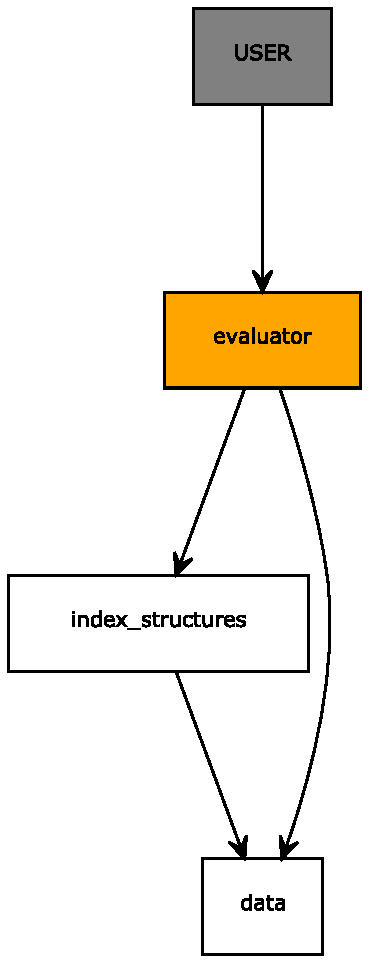
\includegraphics[scale=0.4]{figures/evaluation_framework.pdf}
	\end{center}
	\vspace{-20pt}
	\caption{Modules of Evaluation Framework}
	\label{fig:evaluation-framework}
\end{wrapfigure}

\begin{itemize}
	\item \texttt{data} -- library that contains standard data types used throughout framework and index structures, as well as dataset and test operation generators/loaders
	\item \texttt{index\_structure} -- library that contains all the index structures implemented throughout the project
	\item \texttt{evaluator} -- executable program that takes the index structures, operation lists and other options from the command line and runs a set of automated performance tests that produces timings and profiling (CPU and heap) information
\end{itemize}

The \texttt{evaluator} executable facilitates fast evaluation by allowing multiple index structures to be tested at once, using multiple tests operation lists (as described in Chapter \ref{chap:evaluation-outline}) at once. It stores timings in text files which are fed into bash and Gnuplot scripts to generate plots, which can be understood and incorporated into the report with ease. Figure \ref{fig:evaluation-framework} illustrates the modules of the framework, showing how user performing the performance evaluation only directly interacts with the \texttt{evaluator} executable.

The framework was created because performance analysis would be done very frequently, multiple times per iteration. Manually timing and profiling the code each time is time-consuming and error-prone. Putting more effort initially into creating a system that allows large sets of operations and index structures to be tested at once may save a significant amount of time , especially as many of these performance test are long and must be run multiple times to get averages.

Every index structure defined in the \texttt{index\_structures} module implement the \texttt{IndexStructure} interface, which has the following methods:
\begin{itemize}
	\item \texttt{loadPoints} -- bulk load a collection of points into structure
	\item \texttt{clear} -- remove all points from structure
	\item \texttt{insert} -- insert point into structure (if it's not already stored, see assumption (4) in Section \ref{sec:core-assumptions})
	\item \texttt{remove} -- remove point from structure
	\item \texttt{update} -- modify value of a specific point stored in the structure
	\item \texttt{pointExists} -- equivalent to a point query
\end{itemize}

\subsection{Baseline Implementations}
 
Sequential scan was implemented using the C++ container \texttt{std::vector}, a dynamically resizeable array.  Point queries are performed in $O(n)$ time, as the query iterates through the array sequentially until the given point is found or the end of the array is reached. Inserting a point is $O(1)$ as it is added to the end of the vector. However, Core Assumption (4) from Section \ref{sec:core-assumptions} states all points must be unique in a structure, meaning Sequential Scan must check if a given point exists before inserting it. This is a point query, meaning \texttt{insert} $\in O(n)$. \texttt{delete} is a standard array deletion, making it an $O(n)$ operation.

The octree variant implemented as a baseline is a bucket PR octree. This means the structure partitions the underlying data space into uniformly sized boxes, without using the points as pivots (unlike point quadtrees or kd-trees). It is a bucket octree because \textit{multiple} points can be stored in a single leaf node. The octree dynamically decomposes and composes spatial regions based on its current contents. When the number of points in a leaf node exceeds a certain number, say $M$, then the region represented by the leaf is sub-divided, creating $2^d$ children. The $M + 1$ points are then scattered across the children. Therefore, regions of space that contain more points are decomposed more and sparse regions of space have less granularity, meaning less nodes and memory overhead.

When a point is deleted from a leaf, the contents of the leaf and all of its siblings are checked. If all of these nodes are empty, they are removed and the sub-regions are combined into the original region again. If the now collapsed parent and all of its siblings are empty, then they are collapsed into their parent. This is repeatedly recursively until a parent is reached whose children contain at least one point.

\subsection{Pseudo-Pyramid Tree}

\begin{wrapfigure}[12]{r}{0.5\textwidth}
	\vspace{-40pt}
	\begin{center}
		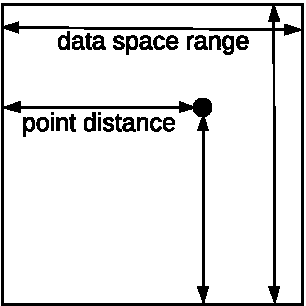
\includegraphics[scale=0.6]{figures/pseudo-pyramid_tree_point_boundary_distances.pdf}
	\end{center}
	\vspace{-20pt}
	\caption{Computing Distance of Point Along Pseudo-Pyramid Tree Boundary Along Each Dimension}
	\label{fig:evaluation-framework}
\end{wrapfigure}

The School of Computing have an implementation of an index structure which is similar to the Pyramid tree, originally written by Zhao Geng\footnote{Z.Geng@leeds.ac.uk}. All the points are stored in a single \texttt{std::vector}. Each point is hashed to an integer representation which acts as the key to a bucket stored in a hash map (specifically \texttt{boost::unordered\_map}). A bucket is a \texttt{std::vector} that contains indices to points in the large point array.

To determine if a point $p$ is stored in the structure, $p$ is first hashed into its one-dimensional representation. The corresponding bucket is then sequentially scanned until the point is found or the end of the bucket is reached. To reduce the number of floating point comparisons, especially for large $d$, the \textit{sums} of each point are stored when they are inserted. This way, a $O(d)$ point comparison needs to be made if the $O(1)$ point sum comparison passes. Simple optimisations were initially made to the original implementation. The original implementation passed many heap allocated structures by-value, resulting in excessive copies and more time being spent allocating memory and copying data. These copies were not necessary and were removed where possible by passing the data by-reference.

In this report, this implementation shall be called the \textbf{Pseudo-Pyramid Tree}. This is because the hashing function used is \textit{inspired} by the Pyramid tree, but is not the same\footnote{There is code to compute the pyramid value of a point in the original code, but curiously it is not used when inserting or querying points. An alternative hashing function was used instead.}. Let $min_i$ and $max_i$ define the minimum and maximum bounds for dimension $i$ and $p$ be a point. To hash $p$, how far along the boundary $p$ is in each dimension is computed using Equation \ref{eq:point-boundary-distance} first. See Figure \ref{fig:point-boundary-distance} for an illustration of what these values mean.

\begin{equation}
	h_i(p) = \frac{p_i - min_i}{max_i - min_i}
	\label{eq:point-boundary-distance}
\end{equation}

Let $B$ be a parameter which controls how likely points will be in the same bucket and let $m$ be a point where $m_i = \ceil{B^{\frac{1}{d}}}$ for $0 \leq i \leq d$. The hashed value $h(p)$ of a point $p$ is then given by Equation \ref{eq:pseudo-pyramid-hash},  where \texttt{toInt} converts a real number to an integer by truncating the decimal part. Computing this is a $O(d^2)$ operation due to the inner loop to compute $\prod_{j=0}^{i}{\lbrack m_j \rbrack}$.

\begin{equation}
	h(p) = \sum_{i = 0}^{d} { \lbrack \texttt{toInt}( h_i(p) \times m_i ) \times \prod_{j=0}^{i}{\lbrack m_j \rbrack} \rbrack }
	\label{eq:pseudo-pyramid-hash}
\end{equation}

Higher $B$ means higher $m$. This increases the magnitude of $h_i(p)$ before it is truncated to an integer, meaning less points will have the same hashed value, meaning less points in the same bucket on average. Lower $B$ will therefore mean more points will be in the same bucket on average.

\subsubsection{Pseudo-Pyramid Tree \texttt{delete}}

The original implementation of the Pseudo-Pyramid Tree did not provide \texttt{delete} and \texttt{update} operations, meaning a \texttt{delete} procedure had to be added. To delete a point $p$, the point is first hashed and the bucket containing the point is found. The index pointing to $p$ in the bucket is removed from the bucket, but the actual point itself is not removed the point array. In other words, the memory is never released until the whole structure is deleted. This makes the structure useful for batch computation because it can be discarded straight after a task, releasing all allocated memory then. However, if the structure is used as part of a long-running process then this is not suitable because there is the potential to run out of memory. This will be referred to as the \textbf{Batch Pseudo-Pyramid Tree} for the rest of this document.

Variants of this structure were implemented to provide a \texttt{delete} operation. The first is the \textbf{Defragmented Pseudo-Pyramid Tree}. When a point's index is deleted from a bucket, the element at the index is marked for deletion from the array at a later time (by adding the index of the point to another \texttt{std::vector}). If the number of marked elements exceeds a certain number $R$, then the $R + 1$ marked elements are erased from the vector (i.e. memory is released). The indices in each bucket are then updated to point to the correct element in the modified array. Even though \texttt{delete} is normally a constant time operation, the worst case is $O(n^2)$ because of this defragmentation procedure.

The \textbf{Rebuild Pseudo-Pyramid Tree} uses a different strategy for releasing memory for unused points. Instead of defragmenting the array by peforming a sequence of array deletions when $R + 1$ elements are marked for deletion, the entire structure is rebuilt. This new cleanup procedure starts by clearing the structure and incrementally building the new structure by only adding points \textit{not} marked for deletion. $n - R$ points will be re-instered and insertion in the worst case is $O(n)$, meaning the worst case complexity of \texttt{delete} is $O((n - R)n)$. The larger $R$ is, the less time it takes to perform this procedure but a larger amount of allocated memory goes unused at a time.

\subsection{Compiler Optimisation}

GCC\footnote{GCC, the GNU Compiler Collection -- \url{http://gcc.gnu.org/}} was the C++ compiler used throughout development and analysis. GCC provides options to automatically modify the source code to make it more efficient on the target platform. There are multiple levels of optimisations, specifying using command line flags, going from 0 (\texttt{-O0} flag, no optimisation) to 3 (\texttt{-O3} flag, maximum optimisation). The default optimisation level is 0. In order to make the structures as fast as possible, level 3 optimisation was used to compile the structures. Table \ref{tab:compiler-optimisation} shows the average execution times for the three operations for each structure, using a 10D random uniformly distributed dataset with 10,000 points. The potential speed gains are huge. For example, the octree's point queries are approximately $6.5$ times faster, just by enabling level 3 optimisation.

\begin{table}
	\centering
	\begin{tabular}{|l|l|l|l|}
		\hline
		\textbf{Structure} & \textbf{Operation} & \texttt{-O0} & \texttt{-O3} \\
		\hline
		\multirow{ 4}{*}{\textbf{Sequential Scan}} & \textbf{Insert} & 1.33509 & 0.111372 \\
		 & \textbf{Delete} & 5.29548 & 0.623759 \\
		 & \textbf{Point Query} & 1.33468 & 0.111909 \\
		\hline
		\multirow{ 4}{*}{\textbf{Octree}} & \textbf{Insert} & 1.23108 & 0.243256 \\
		 & \textbf{Delete} & 0.73156 & 0.13589 \\
		 & \textbf{Point Query} & 0.559736 & 0.0860926 \\
		\hline
		\multirow{ 4}{*}{\textbf{Batch Pseudo-Pyramid Tree}} & \textbf{Insert} & 0.0240852 & 0.00549841 \\
		 & \textbf{Delete} & 0.0108411 & 0.0023433 \\
		 & \textbf{Point Query} & 0.0103358 &  0.00242341 \\
		\hline
		\multirow{ 4}{*}{\textbf{Defragmented Pseudo-Pyramid Tree}} & \textbf{Insert} & 0.0236123 & 0.00558329 \\
		 & \textbf{Delete} & 13.3113 & 1.49306 \\
		 & \textbf{Point Query} & 0.0106464 & 0.00298434 \\
		\hline
		\multirow{ 4}{*}{\textbf{Rebuild Pseudo-Pyramid Tree}} & \textbf{Insert} & 0.0236123 & 0.00558329 \\
		 & \textbf{Delete} & 7.7183 & 0.94745 \\
		 & \textbf{Point Query} & 0.0103173 & 0.00235689 \\
		 \hline
	\end{tabular}
	\caption{Total Execution Time (in Seconds) of Structure Operations With and Without Compiler Optimisations (10D Randomly Uniform  Dataset, 10,000 points used)}
	\label{tab:compiler-optimisation}
\end{table}

While the potential performance boost can be high, there are some downsides to compiler optimisation. Using full optimisaiton can increase the size of the program binaries and it makes the program harder to debug, because the code is restructred and managed, making it difficult to get a method call trace \cite{gcc}. This also makes applications harder to profile. One could profile an application using no optimisation to avoid this issue, but there is no guarantee that functions/methods which are bottlenecks in the non-optimised binary are still bottlenecks in the fully optimised binary. Therefore, optimising the code to remove particular bottlenecks in the non-optimised version may have little, if no, impact on the fully optimised binary (that potentially still performs faster).

To summarise, full compiler optimisation will be used during performance analysis of the structures as the speed gains can be huge. Despite CPU profiling potentially being harder to understand and less useful on fully optimised binaries, this shall still be done over profiling the non-optimised binary because of the aforementioned reasons.

\subsection{Performance Timings}

The structures being analysed in this iteration are sequential scan, octree and the pseudo-pyramid trees (batch and defragmented). $B = 300000$ and $R=3000$ was used as parameters for the Pseudo-Pyramid Trees. This means the Defagmented Pseudo-Pyramid Tree defragments when 3001 elements have been marked for deletion. Table \ref{tab:perf1-randuniform} contains the \textit{total} runtime of \texttt{insert}, \texttt{delete} and point query for uniformly randomly generated points for the analysed structures. When ``-" is shown instead of the number of seconds, it means that the performance test could not finish due to the machine running out of memory. Plots with dimension against execution time are shown for the three operations in Figures \ref{fig:perf1-allinsert-d}, \ref{fig:perf1-alldelete-d} and \ref{fig:perf1-allpquery-d}. The execution times for skewed and clustered data was almost identical to the uniformly random datasets; for the sake of brevity, the tables and plots for these datasets have been placed in Appendix \ref{chap:supp-material}. 

All three plots show that dimensionality has little effect on \textit{insert} and point queries for Sequential Scan. \texttt{delete}'s exeuction time increases as $d$ does, most likely because higher $d$ means more data has to be moved when a point is deleted from the undelying array. As expected, the Octree takes exponentially longer as $d$ increases, due to the exponential increase in nodes at each level ($2^d$ children per node). After $d = 10$ the number of excessive nodes was so high that the performance tests crashed due to there being no more memory to allocate.

Both variants of the Pseudo-Pyramid Tree have the same speed for \texttt{insert} and point queries, which significant outperfoms Sequential Scan and Octree. However, the performance of the trees decreases as $d$ increases and eventually the structure is slower than Sequential Scan (in this case, Sequential Scan starts being faster when $d \approx 57$). This is most likely due to the Pyrmaid Tree's hashing function, which is currently a $O(d^2)$ operation. The $O(n^2)$ defragmentation procedure used by the Defragmented Pseudo-Pyramid Tree causes it to be the slowest structure for deleting points, taking almost twice as long as Squential Scan. The Pseudo-Pyramid Tree on the other hand has the fastest deletion speed, because it only removes the point's index and not the point itself (no expensive memory de-allocations).

Execution times for the 16 dimension dataset of varying size are displayed in Table \ref{tab:perf1-sizevary} and Figures \ref{fig:perf1-allinsert-n}, \ref{fig:perf1-alldelete-n} and \ref{fig:perf1-allpquery-n}. From the plots, it appears the average time it takes to perform a point query and the other operations for Sequential Scan roughly grows linearly with $n$. This is to be expected, due to the complexity of its operations being $O(n)$. The average time for both operations in the Batch Pseudo-Pyramid Tree grows very slowly as $n$ increases. This is likely because an operation's average complexity is $O(d^2)$ and dataset size only affects the performance of these operations if the tree's buckets become crowded with many points (as the buckets have to be searched to find the point). \texttt{delete} in the Defragmented Pseudo-Pyramid Tree grows rapidly as $n$ is increased. Despite the defragmentation procedure being $O(n^2)$, the operation's execution appears to have linear growth (albeit with a higher constant factor than Sequential Scan). Perhaps this worst case bound was simply not reached in the tests, or there is some compiler optimisation at work which reduces this complexity. Considering how inefficient the structure is at deleting points however, the reason will not explored further and focus will be spent on other structures.

Table \ref{tab:perf1-astrophysics} shows the total runtime of different sized samples of the astrophysics dataset, using both operation lists described in Section \ref{sec:timing-operations}.
TODO; do little bit of evaluation

\begin{landscape}

	\begin{table}
		\centering
		\begin{tabular}{|p{2cm}|l|l|l|l|l|l|l|l|l|l|l|}
			\hline
			\textbf{Structure} & \textbf{Operation} & \textbf{1D} & \textbf{2D} & \textbf{3D} & \textbf{5D} & \textbf{8D} & \textbf{10D} & \textbf{30D} & \textbf{50D} & \textbf{100D} & \textbf{200D} \\
			\hline
			\multirow{ 4}{*}{\textbf{Sequential Scan}} & \textbf{Insert} & 0.083928 & 0.0856602 & 0.0858041 & 0.0970701 & 0.0960585 & 0.11025 & 0.13113 & 0.135196 & 0.142939 & 0.142896 \\ & \textbf{Delete} & 0.46229 & 0.577141 & 0.696159 & 0.688754 & 0.634093 & 0.623097 & 0.71913 & 0.882381 & 1.50442 & 3.29082 \\ & \textbf{Point Query} & 0.0834135 & 0.0842911 & 0.0849031 & 0.095202 & 0.0950359 & 0.110287 & 0.130051 & 0.134541 & 0.140541 & 0.142191 \\
			\hline
			\multirow{ 4}{*}{\textbf{Octree}} & \textbf{Insert} & 0.00342762 & 0.0031842 & 0.00361466 & 0.0102806 & 0.0368217 & 0.241889 & - & - & - & - \\ & \textbf{Delete} & 0.00299168 & 0.00256801 & 0.00275838 & 0.00641203 & 0.0259533 & 0.132478 & - & - & - & - \\ & \textbf{Point Query} & 0.00244093 & 0.00213456 & 0.00217879 & 0.00487924 & 0.0229579 & 0.086069 & - & - & - & - \\
			\hline
			\multirow{ 4}{*}{\textbf{Batch Pseudo-Pyramid Tree}} & \textbf{Insert} & 0.00182509 & 0.00201285 & 0.00209451 & 0.00268757 & 0.0040772 & 0.00534821 & 0.0345241 & 0.0927804 & 0.365613 & 1.45883 \\ & \textbf{Delete} & 0.000421524 & 0.000508428 & 0.000604391 & 0.000930548 & 0.00166643 & 0.0023284 & 0.0171595 & 0.0467448 & 0.183702 & 0.728678 \\ & \textbf{Point Query} & 0.000406027 & 0.00050652 & 0.000588536 & 0.00090754 & 0.00173366 & 0.00235772 & 0.0171422 & 0.046788 & 0.183745 & 0.729757 \\
			\hline
			\multirow{ 4}{*}{\textbf{Defragmented Pseudo-Pyramid Tree}} & \textbf{Insert} & 0.00182939 & 0.0019474 & 0.0020951 & 0.00262773 & 0.00407147 & 0.00530696 & 0.0345504 & 0.0927966 & 0.36549 & 1.45541 \\ & \textbf{Delete} & 1.31443 & 1.40514 & 1.48344 & 1.49642 & 1.43011 & 1.48568 & 1.52637 & 1.66116 & 2.21606 & 3.94223 \\ & \textbf{Point Query} & 0.00040555 & 0.000497341 & 0.000604749 & 0.000905514 & 0.00168335 & 0.00233459 & 0.0172749 & 0.046602 & 0.183578 & 0.729738 \\
			\hline
			\multirow{ 4}{*}{\textbf{Rebuild Pseudo-Pyramid Tree}}
			& \textbf{Insert} & TODO & TODO & TODO & TODO & TODO & TODO & TODO & TODO \\
			& \textbf{Delete} & TODO & TODO & TODO & TODO & TODO & TODO & TODO & TODO \\
			& \textbf{Point Query} & TODO & TODO & TODO & TODO & TODO & TODO & TODO & TODO \\
			\hline
		\end{tabular}
		\caption{Total Execution Time (in Seconds) of 10,0000 Structure Operations for Uniformly Random Points}
		\label{tab:perf1-randuniform}
	\end{table}

	\begin{table}
		\centering
		\begin{tabular}{|p{2cm}|l|l|l|l|l|l|l|l|l|}
			\hline
			\textbf{Structure} & \textbf{Operation} & $n = 10$ & $n = 100$ & $n = 1000$ & $n = 5000$ & $n = 10000$ & $n = 50000$ & $n = 100000$ & $n = 500000$ \\
			\hline
			\multirow{ 4}{*}{\textbf{Sequential Scan}} & \textbf{Insert} & 2.38419e-08 & 4.33922e-07 & 9.543899999999999e-07 & 5.56716e-06 & 1.2479999999999999e-05 & 6.64334e-05 & 0.000155559 & 0.001254338 \\ & \textbf{Delete} & 4.0531199999999997e-07 & 1.62601e-06 & 6.87075e-06 & 3.3840599999999996e-05 & 6.77672e-05 & 0.00035017200000000005 & 0.000689738 & 0.00357128 \\ & \textbf{Point Query} & 1.1920899999999999e-07 & 2.5987599999999996e-07 & 8.80718e-07 & 5.5340199999999996e-06 & 1.23303e-05 & 6.42734e-05 & 0.000147421 & 0.001188232 \\
			\hline
			\multirow{ 4}{*}{\textbf{Batch Pseudo-Pyramid Tree}} & \textbf{Insert} & 2.38419e-08 & 2.85149e-06 & 1.24717e-06 & 1.219464e-06 & 1.2071800000000001e-06 & 1.260868e-06 & 1.29801e-06 & 1.4031279999999999e-06 \\ & \textbf{Delete} & 1.3113e-06 & 1.15395e-06 & 5.15223e-07 & 5.222799999999999e-07 & 5.23591e-07 & 6.0327e-07 & 5.8435e-07 & 6.416659999999999e-07 \\ & \textbf{Point Query} & 8.82149e-07 & 1.14202e-06 & 5.06878e-07 & 5.14412e-07 & 5.16725e-07 & 5.48616e-07 & 5.76677e-07 & 6.1645e-07 \\
			\hline
			\multirow{ 4}{*}{\textbf{Defragmented Pseudo-Pyramid Tree}} & \textbf{Insert} & 0.0 & 2.7227399999999996e-06 & 1.23382e-06 & 1.28684e-06 & 1.21651e-06 & 1.290904e-06 & 1.32141e-06 & 1.43266e-06 \\ & \textbf{Delete} & 1.23978e-06 & 1.14918e-06 & 5.09501e-07 & 4.47486e-05 & 0.000149966 & 0.0011255899999999999 & 0.0030419099999999997 & 0.01620092 \\ & \textbf{Point Query} & 7.86781e-07 & 1.14202e-06 & 5.09501e-07 & 5.14174e-07 & 5.17821e-07 & 5.48516e-07 & 5.71394e-07 & 6.18058e-07 \\
			\hline
			\multirow{ 4}{*}{\textbf{Rebuild Pseudo-Pyramid Tree}}
			& \textbf{Insert} & 2.4e-09 & 2.7299e-06 & 1.2047e-06 & 1.1852e-06 & 1.1761e-06 & 1.1957e-06 & 1.2407e-06 & 0.0640399 \\
			& \textbf{Delete} & 1.359e-07 & 1.154e-07 & 1.066e-07 & 2.20697e-05 & 2.96598e-05 & 0.000517846 & 24.9221 & 82.4918 \\
			& \textbf{Point Query} & 6.4e-09 & 2.32e-08 & 5.13e-08 & 5.13e-08 & 5.22e-08 & 2.4e-09 & 2.7299e-06 & 1.2047e-06 \\
			\hline
		\end{tabular}
		\caption{Total Execution Time (in Seconds) of $n$ Operations on an $n$-Sized Structure}
		\label{tab:perf1-sizevary}
	\end{table}

\end{landscape}

\begin{table}
	\centering
	\begin{tabular}{|r|l|l|l|l|}
		\hline
		\textbf{Structure} & \textbf{Operation List} & $n = 10,000$ & $n = 100,000$ & $n = 500,000$ \\
		\hline
		\multirow{ 3}{*}{\textbf{Batch Pseudo-Pyramid Tree}} & \textbf{Insert-Query-Delete} & TODO & TODO & TODO \\
		 & \textbf{Random Operations} & TODO & TODO & TODO \\
		\hline
		\multirow{ 3}{*}{\textbf{Octree}} & \textbf{Insert-Query-Delete} & TODO & TODO & TODO \\
		 & \textbf{Random Operations} & TODO & TODO & TODO \\
		\hline
		\multirow{ 3}{*}{\textbf{Batch Pseudo-Pyramid Tree}} & \textbf{Insert-Query-Delete} & TODO & TODO & TODO \\
		 & \textbf{Random Operations} & TODO & TODO & TODO \\
		\hline
		\multirow{ 3}{*}{\textbf{Defragmented Pseudo-Pyramid Tree}} & \textbf{Insert-Query-Delete} & TODO & TODO & TODO \\
		 & \textbf{Random Operations} & TODO & TODO & TODO \\
		\hline
		\multirow{ 3}{*}{\textbf{Rebulid Pseudo-Pyramid Tree}} & \textbf{Insert-Query-Delete} &  0.571668 & 74.535 & 2104.63 \\
		 & \textbf{Random Operations} & 0.0218163 & 2.79053 & 72.4116 \\
		\hline		
	\end{tabular}
	\caption{Total Execution Time (in Seconds) for Different Sample Sizes of Astrophysics Dataset}
	\label{tab:perf1-astrophysics}
	\end{table}	

\begin{figure}
		\begin{center}
			\begin{subfloat}[\texttt{insert}\label{fig:perf1-allinsert-d}]{%
				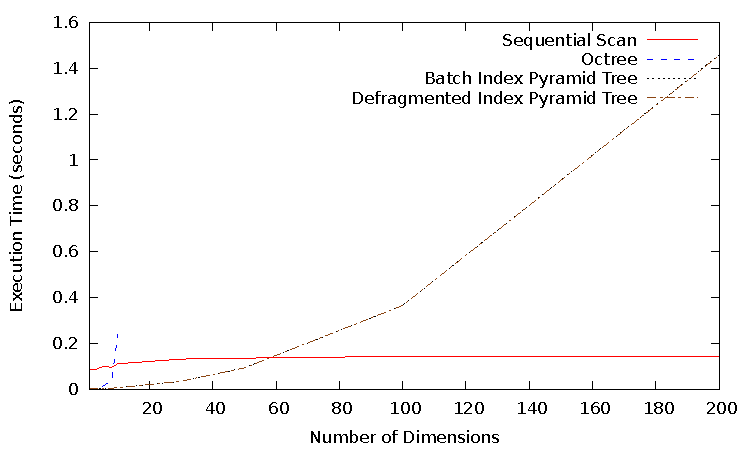
\includegraphics[scale=0.5]{figures/performance_analysis/iteration_1/all_insert_randuniform.pdf}
			}
			\end{subfloat}~
			\begin{subfloat}[\texttt{delete}\label{fig:perf1-alldelete-d}] {%
				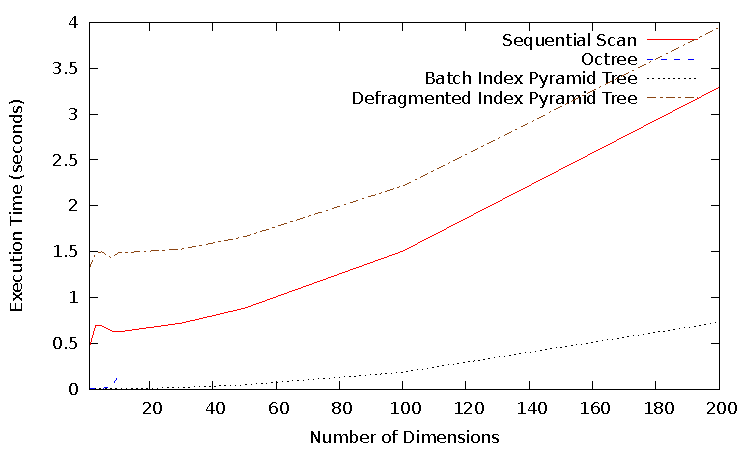
\includegraphics[scale=0.5]{figures/performance_analysis/iteration_1/all_delete_randuniform.pdf}
			}
			\end{subfloat}
			\begin{subfloat}[Point Query\label{fig:perf1-allpquery-d}] {%
				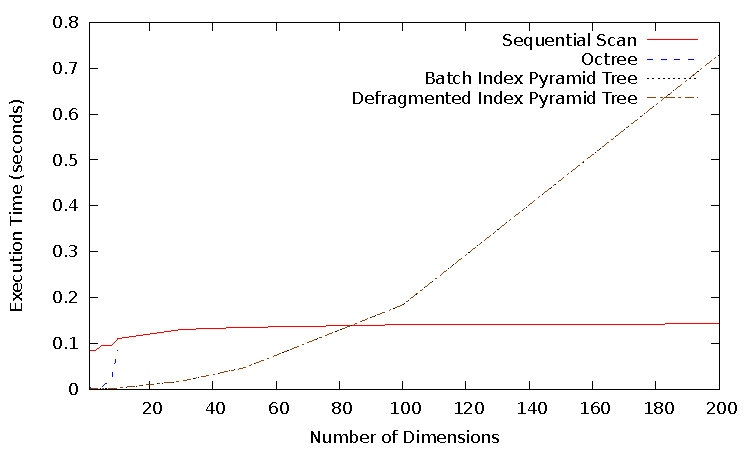
\includegraphics[scale=0.5]{figures/performance_analysis/iteration_1/all_pquery_randuniform.pdf}
			}
			\end{subfloat}  
		\end{center}

		\caption{Performance of 10,000 Operations on Random Uniformly Distributed Datasets of Varying Dimensions}

		\label{fig:perf1-dimensionality}
\end{figure}

% TODO: change plots to total
\begin{figure}
		\begin{center}
			\begin{subfloat}[\texttt{insert}\label{fig:perf1-allinsert-n}]{%
				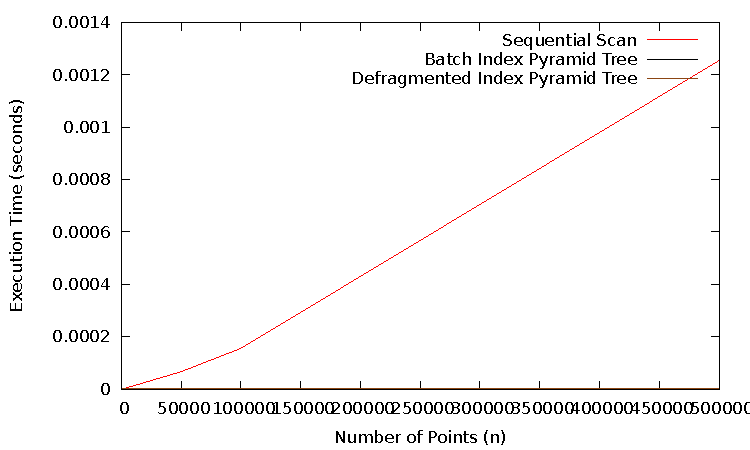
\includegraphics[scale=0.5]{figures/performance_analysis/iteration_1/all_insert_sizevary_average.pdf}
			}
			\end{subfloat}~
			\begin{subfloat}[\texttt{delete}\label{fig:perf1-alldelete-n}] {%
				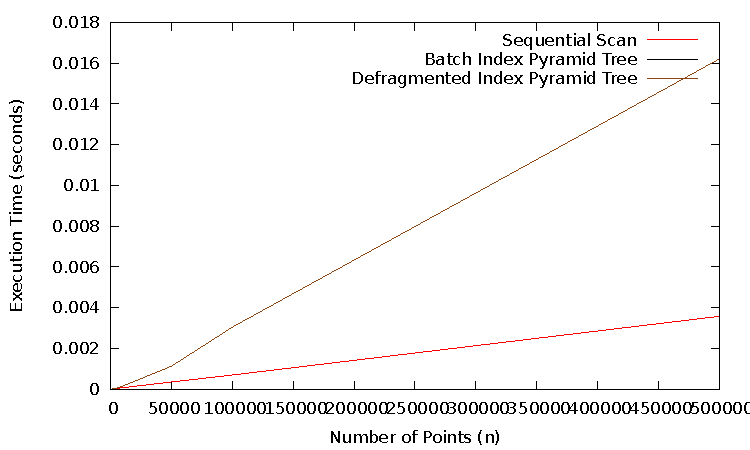
\includegraphics[scale=0.5]{figures/performance_analysis/iteration_1/all_delete_sizevary_average.pdf}
			}
			\end{subfloat}
			\begin{subfloat}[Point Query\label{fig:perf1-allpquery-n}] {%
				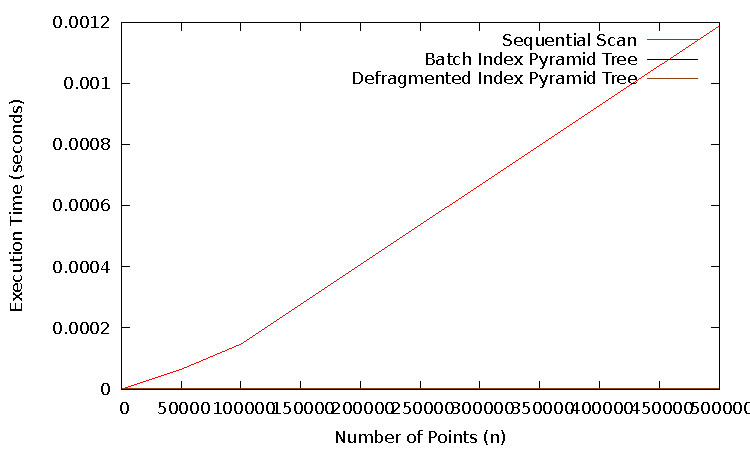
\includegraphics[scale=0.5]{figures/performance_analysis/iteration_1/all_pquery_sizevary_average.pdf}
			}
			\end{subfloat}  
		\end{center}

		\caption{Average Operation Performance on Random Uniformly Distributed Datasets of Varying Dimensions}

		\label{fig:perf1-size}
\end{figure}

\subsection{Profiling Results}

CPU and heap profiling was performed on each structure to determine where the performance bottlenecks are and how much memory each structure uses. Table \ref{fig:perf1-profiling} shows which functions took the majority of the execution time for each structure, as well as how much heap memory the structure consumed when storing all of the input dataset's points. The dataset used contained 10,000 10D uniformly random points and the CPU profiling was performed over the Insert-Query-Delete operation list.

\begin{table}
	\centering
	\begin{tabular}{|p{6cm}|p{6cm}|p{2.5cm}|}
		\hline
		\textbf{Structure} &
			\textbf{Dominant Functions (\% time spent on average)}
		& \textbf{Total Heap Memory Used} \\
		\hline
		\textbf{Sequential Scan} & 
			\begin{tabular}{l} \texttt{Point::operator==()} (63.3\%) \\ \texttt{std::vector::remove()} (21.6\%)
			\end{tabular}
			& 0.9 MB \\
		\textbf{Octree} & \texttt{subdivide()} (34.4\%) & 291.3 MB \\
		\textbf{Batch Pseudo-Pyramid Tree} & \texttt{hashPoint()} (99.7\%) & 1.5 MB \\
		\textbf{Defragmented Pseudo-Pyramid Tree} & \texttt{defragment()} (72.7\%) & 2.2 MB \\
		\textbf{Rebuild Pseudo-Pyramid Tree} & \texttt{rebuild()} (52.49\%) & 3.5 MB \\
		\hline
	\end{tabular}
	\caption{Function Bottlebecks and Total Heap Memory Used for 10,000 10D Points}
	\label{fig:perf1-profiling}
\end{table}

Sequential Scan's core bottleneck was the point equality checking function, taking approximately 63.3\% of the structure's total execution time. This is unsurprising, considering the algorithm. To check a given point exists, the structure iterates through the stored points and compares them with the given one. In the worst case, $n$ point comparisons are made for each operation, where $n$ is the number of points stored. Therefore, frequency of these comparisons is high, meaning the sum of the individual comparisons times consume most of the execution time. Octree performs multiple heap allocations and region checks when sub-dividing leaf nodes, which is biggest cause of slowdown.

Since hash table operations are $O(1)$ on average, the Batch Pseudo-Pyramid Tree spends very little time searching the underlying hash table structure. The vast majority of the structure's time is spent hashing $d$-dimensional points to an integer value. The slowest of the four structures, the Defragmented Pseudo-Pyramid Tree, spends most of its time defragmenting the underyling point array. The expensive $O(n^2)$ defragmentation steps means \texttt{delete} dominates the other operations.

Sequential Scan uses the least heap memory, because it only stores the points and contains no overhead. The Pseudo-Pyramid Tree stores buckets and point sums to accelerate search, which is the reason it uses more heap memory than Sequential Scan. Even though only 10,000 10D points are stored in the octree, almost 300 MB of memory is used. A non-leaf octree node has $2^d$, which means the memory overhead increases exponentially as $d$ does. When $d = 10$, each non-leaf has 1024 children. Due to the curse of dimensionality and data sparseness \cite{data-sparseness}, it is likely the majority of these nodes will be empty, meaning a significant number of excessive nodes and memory is being used.

TODO: rebuild

\subsection{Summary}

This iteration implemented the two baselines, Sequential Scan and Octree, as well as a hash table based Pyramid Tree. These structures have been timed to determine how the structures' performance behaves as the dimensionality and dataset size increases. Sequential Scan is highly inefficient for large $n$, but mostly remains unaffected by high $d$. The Octree is essentially unusable for high dimensions because of the $O(2^d)$ spatial complexity, which causes the machine to run out of memory almost immediately. Furthermore, the plots show that execution time of the operations also increases exponentially as $d$ increases.

The Batch Pseudo-Pyramid Tree provides very fast performance on all operations, but becomes slower when a certain number of dimensions is reached ($\approx 57$). CPU profiling has shown that this is most likely to do with the $O(d^2)$ hash function, where the majority of the structure's execution time is spent. Furthermore, the Batch pyramid tree does not release the memory of deleted points. The Defragmented Pseudo-Pyramid Tree is a variant of the Batch Pseudo-Pyramid Tree which occasionally performs an $O(n^2)$ defragmentation procedure to release memory. Tests have shown this to be inefficent, being even slower than Sequential Scan's \texttt{delete}.

Despite difficulties releasing memory and a troublesome hashing function, the Pseudo-Pyramid Tree shows great promise as a structure capable of dealing with high-dimensional data. It was decided that focus of the next iteration would be modifying the Pyramid tree implementation to provide two things: a more efficient \texttt{delete} that also releases memory and a faster hashing function to provide further speedup and allow the structure to be used for even higher dimensions.